\documentclass[11pt]{article}
\usepackage{geometry}                
\geometry{letterpaper}                   
\usepackage[utf8]{inputenc}
\usepackage{graphicx}
\usepackage{sidecap}
\usepackage[hang]{caption}
\usepackage{amssymb}
\usepackage{epstopdf}
\usepackage{booktabs}
\usepackage{mcode}
\usepackage{url}
\usepackage[numbers]{natbib}
\usepackage{amssymb, amsmath ,empheq}
\usepackage{lmodern}
\usepackage[labelfont={bf,small},font={small},aboveskip=1.2em,belowskip=0em]{caption}
\graphicspath{{figures/}}
\setlength{\parindent}{0px}

\usepackage{listings}
\lstset{
basicstyle=\footnotesize,  
% keywordstyle=\color{blue},       		
  title=\lstname,  				
 numbers=left,                    			
 breakatwhitespace=false,
 breaklines=true
}
\definecolor{background}{RGB}{248,248,255}
\definecolor{dunkelblau}{RGB}{77,77,94}
\definecolor{black}{gray}{0} % 10% gray
\DeclareCaptionFont{white}{\color{white}}
\DeclareCaptionFormat{listing}{\colorbox{dunkelblau}{\parbox[b][0.375cm]{\textwidth-2\fboxsep}{\hspace{15pt}#1#2#3}}}
\captionsetup[lstlisting]{format=listing,labelfont=white,textfont=white, belowskip=0pt,aboveskip=0pt, singlelinecheck=false, margin=0pt,  font={bf, footnotesize}}
\usepackage[percent]{overpic}
\begin{document}
\lstset{
  numbers=left,                   % where to put the line-numbers
  numberstyle=\tiny\color{darkgray},  % the style that is used for the line-numbers
  stepnumber=1,               % Abstand zwischen den Zeilennummern
  numbersep=10pt,              % Abstand der Nummern zum Text
  tabsize=2,                  % Groesse von Tabs
  extendedchars=true,         %
  breaklines=true,            % Zeilen werden Umgebrochen
  showspaces=false,           % Leerzeichen anzeigen ?
  showtabs=false,             % Tabs anzeigen ?
  xleftmargin=17pt,
  language=Matlab,
  framexleftmargin=17pt,
  framexrightmargin=0pt,
  framexbottommargin=4pt,
  backgroundcolor=\color{background},
  showstringspaces=false,      % Leerzeichen in Strings anzeigen ? 
  frame=b,
  basicstyle=\scriptsize\ttfamily
}


\thispagestyle{empty}

\begin{center}

\includegraphics[width=5cm]{ETHlogo.pdf}

\bigskip


\bigskip


\bigskip


\LARGE{ 	Lecture with Computer Exercises:\\ }
\LARGE{ Modelling and Simulating Social Systems with MATLAB\\}

\bigskip

\bigskip

\small{Project Report}\\

\bigskip

\bigskip

\bigskip

\bigskip

\bigskip

\begin{center}
\textbf{\huge{Predicting Traffic Jam}}\\ \vspace{.2cm}
\textbf{\huge{at Gotthard}}\\
\end{center}
\bigskip

\bigskip

\vspace{1cm}

\Large{Eric Hayoz, Janick Zwyssig}



\bigskip

\bigskip

\bigskip

\bigskip

\bigskip

\bigskip

\bigskip
\vspace{3cm}

Zurich\\
December 2014\\

\end{center}



\newpage

%%%%%%%%%%%%%%%%%%%%%%%%%%%%%%%%%%%%%%%%%%%%%%%%%

\newpage
\section*{Agreement for free-download}
\bigskip


\bigskip


\large We hereby agree to make our source code for this project freely available for download from the web pages of the SOMS chair. Furthermore, we assure that all source code is written by ourselves and is not violating any copyright restrictions.

\begin{center}

\bigskip

\bigskip
\begin{minipage}[t]{.4\textwidth}\centering
Eric Hayoz\\ \vspace{.1cm}

\includegraphics[height=1cm]{ehayoz.png}
\end{minipage}
\begin{minipage}[t]{.4\textwidth}\centering
Janick Zwyssig\\ \vspace{.1cm}

\includegraphics[height=1cm]{jzwyssig.png}
\end{minipage}
\end{center}
\newpage
%%%%%%%%%%%%%%%%%%%%%%%%%%%%%%%%%%%%%%
\begin{overpic}[width=\textwidth, clip=true, trim=1cm 3.9cm 1cm 1cm]{originality.pdf}
\put(34,7){
\includegraphics[height=.2cm]{ehayoz.png}}
\put(66,7){
\includegraphics[height=1.02cm, angle=180, origin=c]{jzwyssig.png}}
\end{overpic}
\clearpage
%%%%%%%%%% Table of content %%%%%%%%%%%%%%%%%

\tableofcontents

\newpage

%%%%%%%%%%%%%%%%%%%%%%%%%%%%%%%%%%%%%%%



\section{Abstract}

\textit{Abstract of Eric Hayoz \& Janick Zwyssig, Modelling the phenomenon of congestion at Gotthard -- A case study, 2014:}

This work describes the modelling of congestion on the stage between Erstfeld and the Gotthard tunnel in Göschenen, in the canton of Uri. In a first step a simulation based on the Nagel-Schreckenberg model was created. The model was supplemented by a second lane, a red-light and the ability to change the lane. A mapping from real data to the model allows to compare values. 
The main goal is to train the model that one can compare the measured congestion to a real traffic jam. For that the authors have implemented a congestion measurement and have processed datasets, provided by ASTRA (Amt für Strassen). A parameter setting that fits the reference data best was found. 

Finally the trained model was feed by two other, unused datasets to compare the results. Unfortunately, due to abnormalities of the datasets and some restrictions of the model there are big deviations to reference data. 

\section{Individual contributions}

We devided the code work as follows:

Eric Hayoz:
\begin{itemize}
\item Implementation NaSch-Modell for 2 cars 
\item Handling Dataset with inFlow and Speed 
\item Correlation Reality - Model
\item Creating optiFinder 
\end{itemize}

Janick Zwyssig:
\begin{itemize}
\item Implementation NaSch-Modell for n cars
\item Implementation laneChange \& redLight
\item curve fitting for results
\item congestion measurement
\end{itemize}

At the end both authors were involved in every part. The article was performed together.

\section{Introduction}

Nowadays, traffic jams belongs to every day life. Because Switzerland is an important transit way to Southern Europe for traffic, the Gotthard tunnel becomes to an unavoidable bottleneck. The tunnel stretches out over 15 Kilometers from Göschenen, Kanton Uri to Airolo in the canton of Ticino. Over and over again it comes to long traffic jams, at peak times up to 20 Kilometers. Responsible for that are  on the one hand holidays in Switzerland or neighbor countries and on the other hand the lane reduction from two to one lane. Switzerland has been discussing for many years about this issue and building a second tunnel. The purpose of the second tunnel should be built for security reasons an not in order to increase the traffic flow. This is due to an election 20 years ago, called the Alpenschutzinitiative. 
In near future there will be a restauration for the tunnel. That's why the discussion about a second tunnel will go on again.

The authors have the goal to investigate the Gotthard tunnel on the north side in Göschenen. That's why a model has been created. By means of the number of cars passing through Erstfeld (a village 19 Kilometers distance from the tunnel), the length of congestion can be measured. The Nagel-Schreckenberg model will be employed for the simulation.


\subsection{Motivation}
As one of the authors is born in the canton of Uri he knows about the traffic issues at the Gotthard tunnel. This explains the personal motivation to investigate the phenomenon of traffic congestions. The other author is often on the way by car, he has already wasted a lot of time in traffic congestions
and thus has also a burning interest in efficient solutions to handle them.

















\section{Description of the Model}

\subsection{The Nagel-Schreckenberg model}
This model was created in the 90s by the German physicists Kai Nagel and Michael Schreckenberg to simulate 
traffic flow on highways. It explained the so called \textit{Phantom-Congestion} which occurs when drivers 
linger by not accelerating even if they have the opportunity to do so.

The model is a cellular automata based on four very simple rules, which are applied in sequence. One complete loop is called an iteration.

\begin{enumerate}
\item Acceleration: Each vehicle, that has not yet reached the maximum speed (which is 5), increases its speed by one unit.
\item Deceleration: If the size of the gap (in cells) between two vehicles is less than the speed of the following car (in speed units), this cars speed is reduced to a value equivalent to the size of the gap.
\item Lingering: Every vehicle reduces its speed by 1 with a probability $p$ $(0 \leq p \leq 1)$.
\item Moving forward: Every vehicle moves forward the number of cells equal to its speed.
\end{enumerate}

\subsection{Example of an iteration}
\begin{figure}[H]
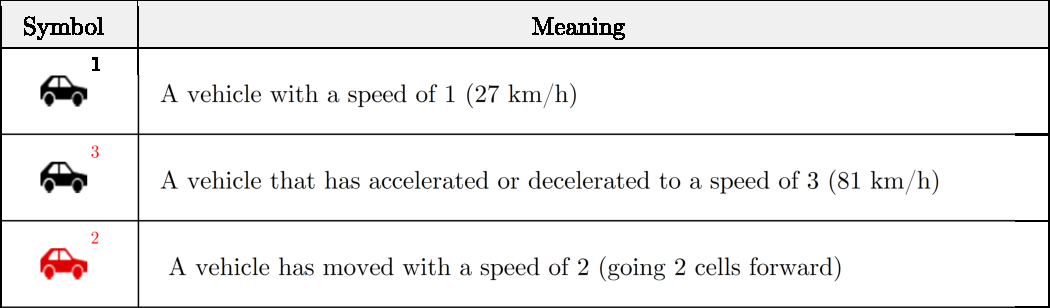
\includegraphics[width=\textwidth]{nasch_symbol.pdf}
\caption{Nagel-Schreckenberg model -- Symbols}
\end{figure}

Random startup setting for time \textit{t}\\ \vspace{-.2cm}

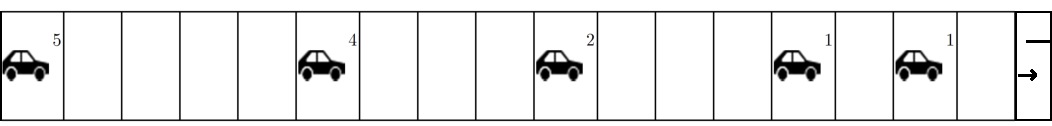
\includegraphics[width=\textwidth]{nasch_1.pdf}

\vspace*{1cm}

Step (1) -- Acceleration, $v_{max} = 5$\\ \vspace{-.2cm}

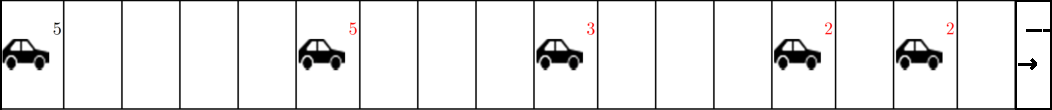
\includegraphics[width=\textwidth]{nasch_2.pdf}\vspace*{1cm}
\\
Step (2) -- Deceleration\\ \vspace{-.2cm}

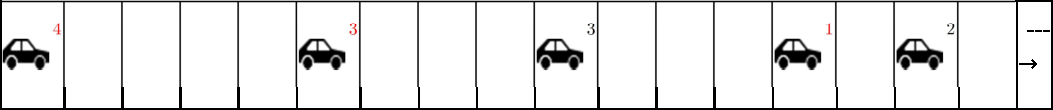
\includegraphics[width=\textwidth]{nasch_3.pdf}\vspace*{1cm}

Step (3) -- Lingering ($\rho = 1/3$, affecting the two leading cars)\\ \vspace{-.2cm}

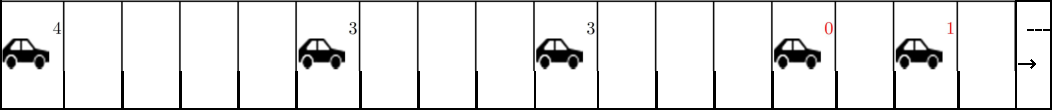
\includegraphics[width=\textwidth]{nasch_4.pdf}\vspace*{1cm}

Step (4) -- Moving (Setting for the time \textit{t + 1})\\ \vspace{-.2cm}

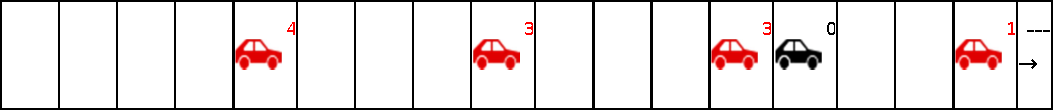
\includegraphics[width=\textwidth]{nasch_5.pdf}



\subsection{Situation}
The distance between Erstfeld and the Gotthard tunnel is relevant for the model. The highway to the tunnel is two-laned and will be reduced to one lane in front of the tunnel. As on the figure \ref{sketch} shown, the authors resigned to depicted any exits. The reason for this is first to reduce complexity of the model and second to neglect irrelevant factors. In case of congestion there is a red light that regulates the traffic flow, which is also taken into account in the model. 

\begin{figure}[h]\centering
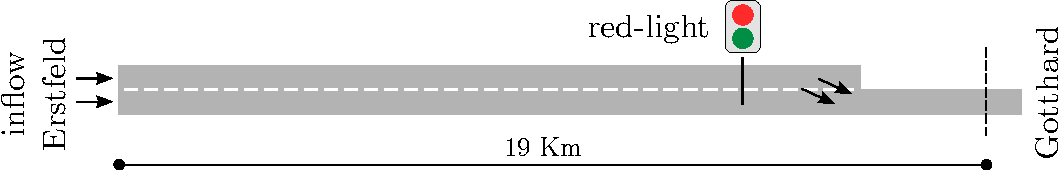
\includegraphics[width=.9\textwidth]{sketch.pdf}
\caption{Sketch of model}
\label{sketch}
\end{figure}

\begin{figure}[h]\centering
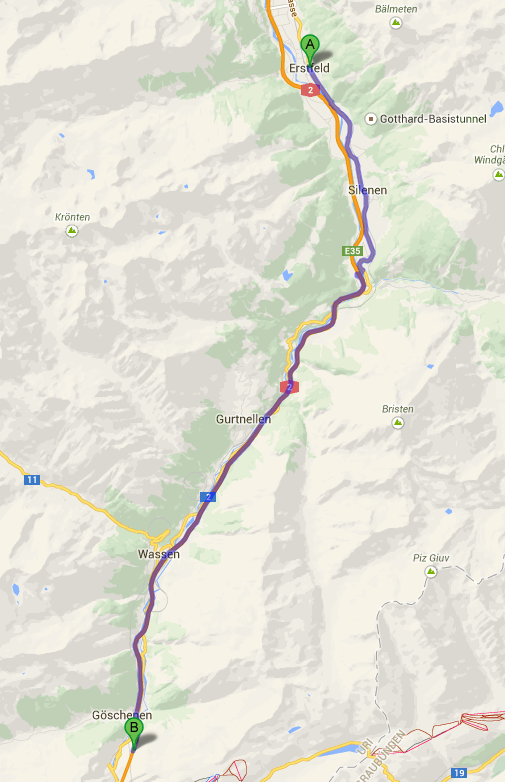
\includegraphics[angle=90, width=.7\textwidth]{map.png}
\caption{map of Uri, A: Erstfeld, B: Gotthard tunnel at Göschenen}
\label{map}
\end{figure}


\section{Implementation}




\subsection{Correlation between reality and model}

\small{
\begin{tabular}{p{0.32\textwidth} p{0.4\textwidth} p{0.21\textwidth}}
\textbf{Item}			& \textbf{Reality}	&  \textbf{Model}\\
\midrule
Time			& 1s		& 1 iteration\\
Maximum speed	& 120  km/h (we defined vmax as 100 km/h to get even values) & 5 (only 6 levels)\\
Length of an average car (Skoda Octavia) & 4.5 m & 1 cell\\
Distance Erstfeld - Göschenen & 19'000 m & 4222 cells (19'000 m / 4.5 m, rounded)
\end{tabular}

\vspace*{1.5cm}
\begin{tabular}{p{0.22\textwidth} p{0.49\textwidth} p{0.22\textwidth}}
\textbf{Variable name}	& \textbf{Meaning}	& \textbf{Values} \\
\midrule
moveProb & Probability for a car to move forward & 0\ldots 1  \\
moveCorr & Modify moveProb for a given time (in order to improve congestion length prediction) &  -1\ldots 1\\
laneChange & Probability for a car to change its lane & 0\ldots 1\\
- & Value of laneChange as a function of distance to changeCell (for locations where cars have to change from left to right) & Constants in equation\\
redLight & Illuminate a dropcounter redlight in front of tunnel (it turns on if congestion length $>$ 2 km and redLight is set to 1) & 0, 1\\
dropCounter & Length of a period when redlight is ON & 0\ldots Inf \\
- & Maximum speed just in front of tunnel & 0\ldots 5
\end{tabular}
}

\subsection{Inflow}
The inflow is given in \#cars / 180 s. For every iteration in our model, the cars are spawned in Erstfeld (starting position) on the two lanes with a total probability $p = \#\textrm{cars} / 180$. As there are normally slightly more vehicles on the right lane, we multiply $p$ for the right lane with a factor of 1.1 and the $p$ for the left lane with a factor of 0.9.

\subsection{Average speed}
First we convert the average speed from km/h (0\ldots 120) to “Nagel-Schreckenberg-Speed” (0\ldots 5). If the speed is more than 5, we round down to 5.
Example:

Average Speed is 94 km/h. Converting into Nagel-Schreckenberg-Speed results in 4.7. Our model would in this case spawn 70\% of the cars with a speed of 5, and 30\% with a speed of 4.

\subsection{Lane Change and red-light}
As cars change lane often in reality, it should be also a part of the model. Furthermore it is necessary to change the lane due to lane reduction in front of the tunnel. The probability to change the lane from left to the right is higher than backwards. That yields more cars on the right lane. In front of the tunnel the probability increases, due to lane reduction.

Red-light is activated if the congestion length exceed the length of one Kilometre. It's acting approximately 40 meters in front of the lane reduction. Every second one car can pass through the tunnel. 


\subsection{Congestion Length}
The length of a congestion is given in Kilometres. First we calculate the length of the congestion in our simulation and then multiply the length (unit: cells) by the length of a cell (4.5 m) to enable a comparison between the virtual (calculated) congestion with the real (measured) congestion.

Measuring the congestion length in our model: To obtain a stable output, we divide the highway into blocks with a length of 50 cells. If a block fulfils the two following criteria, it is declared a congestion block: high density and low average speed. We count the congestion blocks starting in Göschenen heading northbound to Erstfeld, and we only accept one uncongested block between any two blocks, otherwise we consider the congestion as terminated at the point where two or more blocks do not fulfil the congestion criteria anymore.


\subsection{Processing the datasets delivered by ASTRA}
The attached extract shows among other things that we have information about the inflow values and average speeds in 3 minutes intervals. We also have the length of the congestion at specific times (random times and course measurements). These are the three values that we used.

\begin{figure}[h]
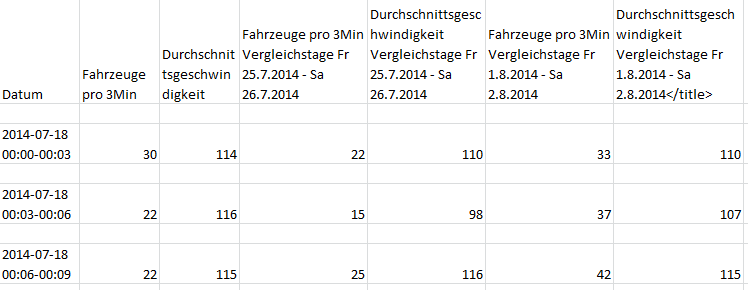
\includegraphics[width=\textwidth]{dataset.png}
\caption{Inflow values with average speeds}
\end{figure}

\begin{figure}[h]
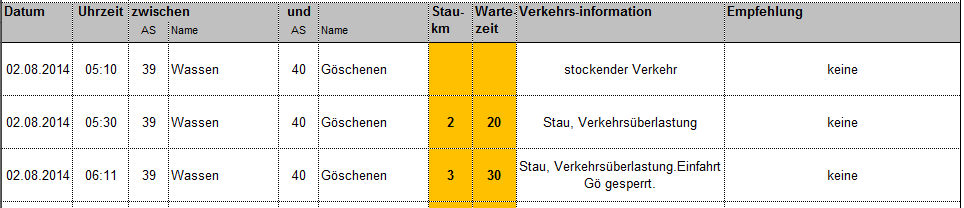
\includegraphics[width=\textwidth]{congestion.png}
\caption{Congestion data}
\end{figure}


\section{Simulation Results and Discussion}


The reference data for congestion measurement is provided by ASTRA (Bundesamt für Strassen). There are four datasets: 
\begin{itemize}
\item Dataset 1: measurement of 2014 July, 18. - 19.
\item Dataset 2: measurement of 2014 August, first
\item Dataset 3: measurement of 2014 July, 25. - 26.
\item Dataset 4: measurement of 2014 August, second
\end{itemize}

In a first step the model will be trained by dataset 1 and 2. The authors wrote a program which calculates specified values of a specified variable (moveProb and moveCorr) for a given number of times. With other words, it finds the optimal parameter values that minimizes the error of measured congestion. In a second step, the datasets 3 and 4 are used to evaluate the previous trained model.

\subsection{Preparing dataset -- curve fitting}
The timestamps for the measurement are irregular. In order to compare the congestion from the model to the reference data, the breakpoints will be interpolated. The resulting curve can be used to generate regular timestamps for measurement. The authors have decided to go for a linear interpolation. That means that every point will be connected by a straight line with its neighbour, see on the figures below. A linear interpolation is reasonable, because the congestion length between two breakpoints can't change very quickly.

%Die Referenzdaten vom ASTRA (Bundesamt für Strassen) enthalten Staumessungen. Diese sind in unregelmässigen Abständen gemessen. Um einen Vergleich mit der Messung im Modell 
%vorzunehmen, werden die Datenpunkte Interpoliert. Die gefundene Kurve wird dann benutzt, um regelmässige Messungen zu generieren. Die Authoren haben sich für eine lineare %Interpolation entschieden, sodass Punkt zu Punkt mit einer Geraden verbunden wird. Dies ist sinnvoll, weil die Länge des Staus zwischen zwei Punkten nur geringfügig ändern kann.

\begin{figure}[h]\centering
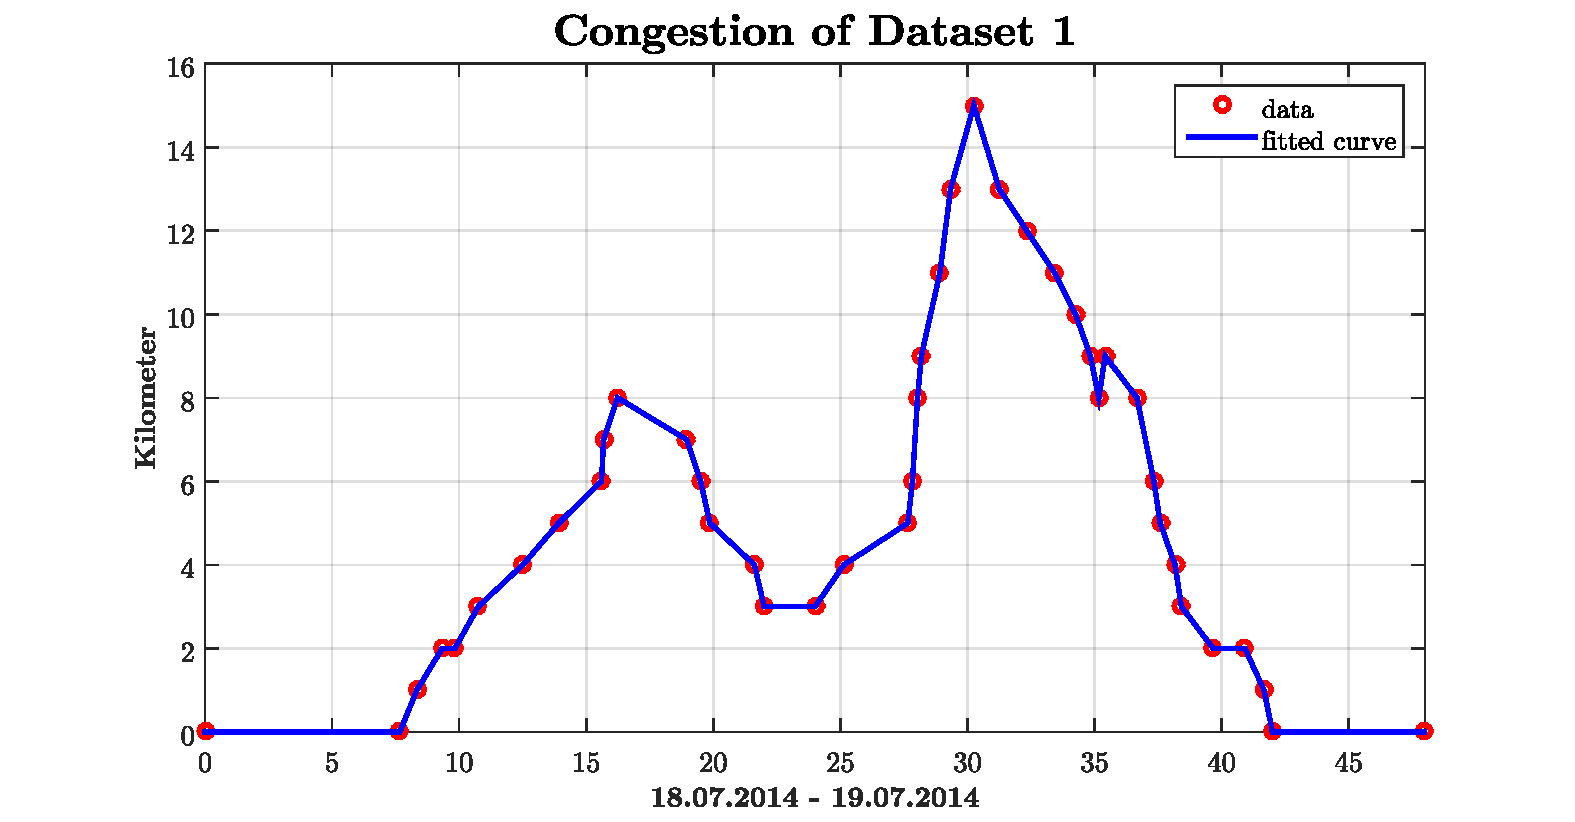
\includegraphics[width=.9\textwidth]{dataset1.pdf}
\caption{Dataset 1}
\end{figure}

\begin{figure}[h]\centering
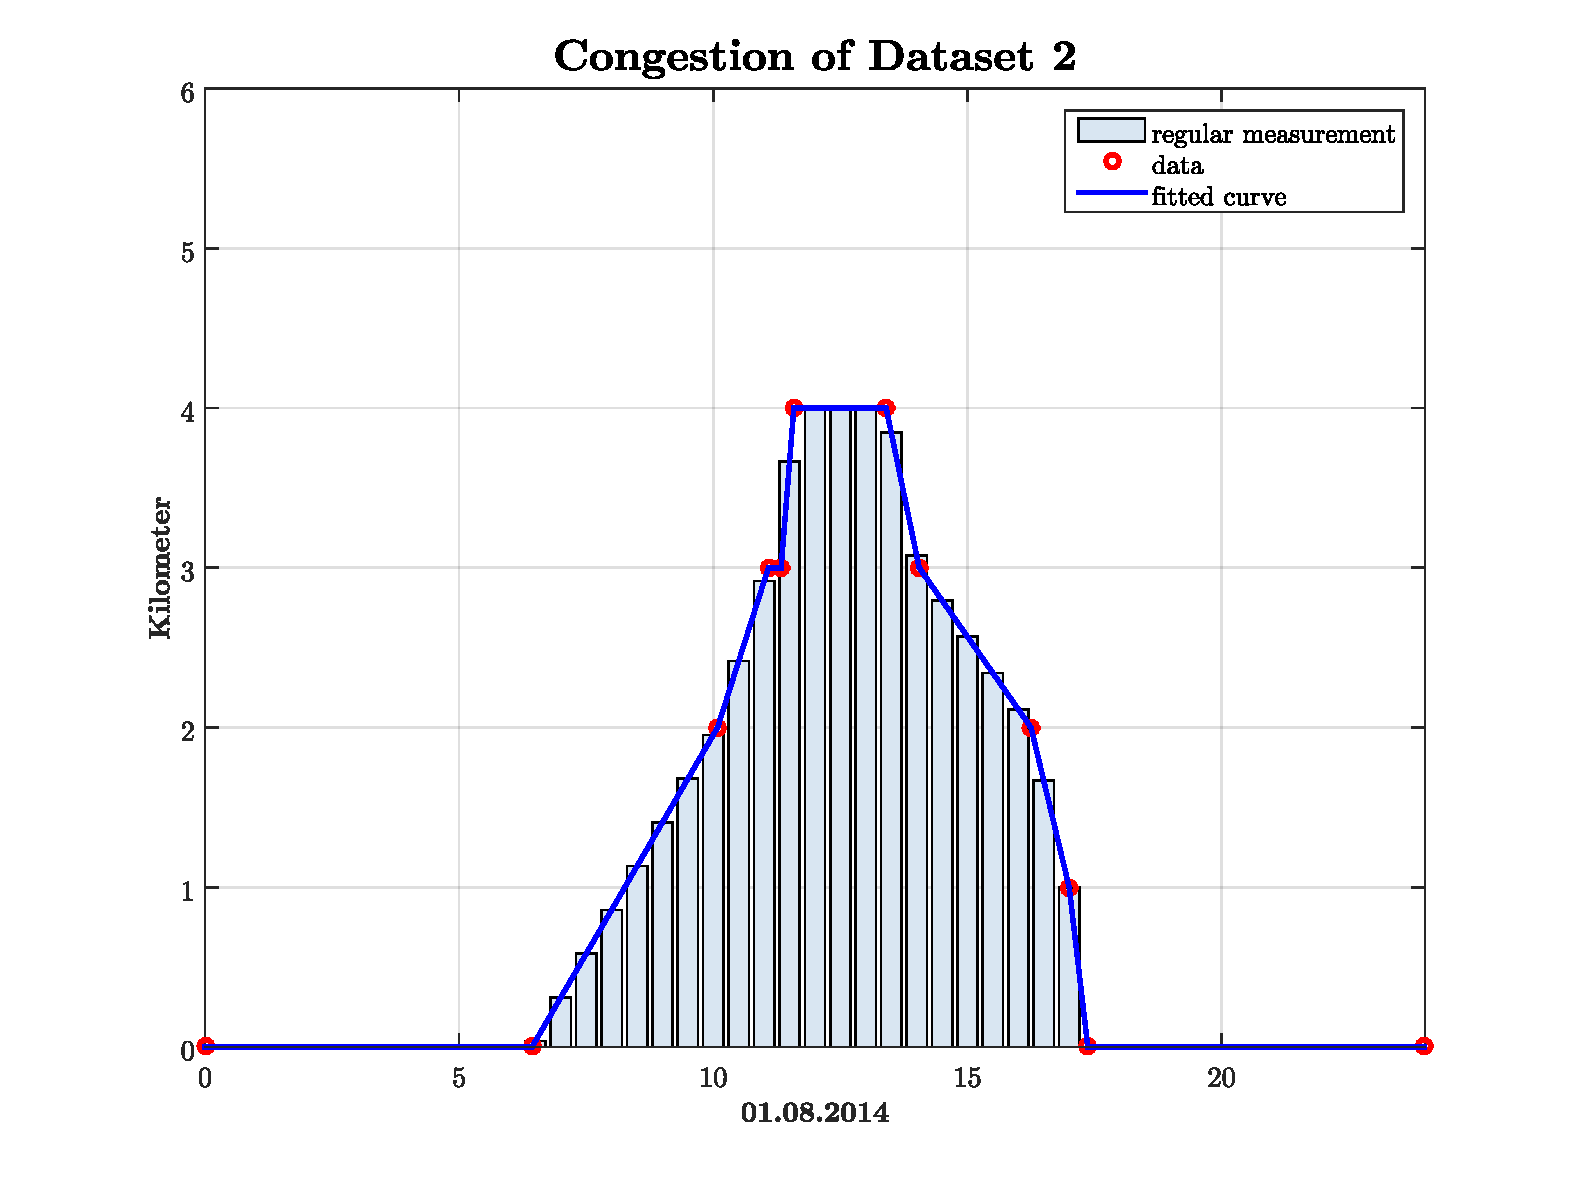
\includegraphics[width=.9\textwidth]{dataset2.pdf}
\caption{Dataset 2, added regular measurements for comparison}
\end{figure}

\subsection{train model}
\newpage

\section{Summary and Outlook}

The authors created a model based on the "Nagel-Schreckenberg-Modell". It was extended to fit the situation at the
"Gotthard-Strassentunnel Nordportal" between Erstfeld and Göschenenen. Its purpose is to predict traffic congestions in
front of the tunnel.

The model was firstly trained with two datasets (24h and 48h), which were both provided by ASTRA.

The authors soon realised that there were some uncasualities in the congestion plot diagrams, which lead back to
measuring mistakes or inaccuracy of the dataset.

At the very end, the finished model had to prove its accuracy by predicting traffic congestions with two other datasets
(24h and 48h, also provided by ASTRA), which have not been used before.


\section{Appendix}
\section*{Code}


\lstinputlisting[linerange=1-100, caption=Matlab-code]{../../code/final.m}

\begin{thebibliography}{9}

\bibitem{trafficflow}{
	Andreas Schadschneider.
\newblock \textit{Traffic flow modelling}.
\newblock \url{http://www.thp.uni-koeln.de/~as/Mypage/traffic.html}.
\newblock April 2000

}

\bibitem{nasch}{
	Torsten Held, Stefan Bittihn.
\newblock \textit{Cellular automata for traffic simulation -- Nagel-Schreckenberg model}.
\newblock March 2011
}

\bibitem{nasch2}{
	K. Nagel and M. Schreckenberg.
\newblock \textit{A cellular automaton model for freeway traffic}.
\newblock 1992
}

\end{thebibliography}











\end{document}  



 
